\documentclass[compress,xcolor=dvipsnames]{beamer}
\usepackage{ifthen}
\usepackage{tikz}
\usepackage{calc}
%\usetikzlibrary{decorations.pathreplacing}
\usepackage{times}
\usepackage{soul}
\usepackage{pifont}
\usepackage[super]{nth}
\usetikzlibrary{decorations.pathmorphing}
\usepackage{martonsdefs,martonsthms}

\graphicspath{{/home/mb13434/latex/packages/}{/home/balazs/latex/packages/}}

% Animate master
\newcount\a
\newcounter{xal}
\newcounter{xar}
\newcounter{xbl}
\newcounter{xbr}
\newcounter{xcl}
\newcounter{xcr}
\newcounter{xdl}
\newcounter{xdr}
\newcounter{xel}
\newcounter{xer}
\newcounter{xfl}
\newcounter{xfr}
\newcounter{xgl}
\newcounter{xgr}
\newcounter{xhl}
\newcounter{xhr}
\newcounter{xil}
\newcounter{xir}
\newcounter{l}

\useoutertheme{split}
\usecolortheme{dolphin}

\setbeamertemplate{navigation symbols}{}
\setbeamertemplate{footline}{}

\setbeamercolor{palette primary}{use=structure,bg=structure.fg!70!black,fg=white}
\setbeamercolor{subtitle}{fg=Orange}

\setbeamercolor{expl}{fg=YellowOrange}
\setbeamercolor{blackk}{fg=Black}
\newcommand*{\blackk}[1]{{\usebeamercolor[fg]{blackk}#1}}
\setbeamercolor{gr}{fg=Gray}
\newcommand*{\gr}[1]{{\usebeamercolor[fg]{gr}#1}}
\setbeamercolor{olgr}{fg=OliveGreen}
\newcommand*{\olgr}[1]{{\usebeamercolor[fg]{olgr}#1}}
\setbeamercolor{cola}{fg=Black!\thecga!averagebackgroundcolor}
\newcommand*{\cola}[1]{{\usebeamercolor[fg]{cola}#1}}
\setbeamercolor{colb}{fg=Black!\thecgb!averagebackgroundcolor}
\newcommand*{\colb}[1]{{\usebeamercolor[fg]{colb}#1}}
\setbeamercolor{colc}{fg=Black!\thecgc!averagebackgroundcolor}
\newcommand*{\colc}[1]{{\usebeamercolor[fg]{colc}#1}}
\setbeamercolor{colab}{fg=Black!\thecgab!averagebackgroundcolor}
\newcommand*{\colab}[1]{{\usebeamercolor[fg]{colab}#1}}
\setbeamercolor{colbc}{fg=Black!\thecgbc!averagebackgroundcolor}
\newcommand*{\colbc}[1]{{\usebeamercolor[fg]{colbc}#1}}


\title{
 Local convergence in t-PNG
}
\author{M\'arton Bal\'azs}
\subtitle{\small joint with Ruby Bestwick, Artem Borisov, Elnur Emrah, and Jessica Jay}
\date{Universality in the Kardar-Parisi-Zhang class and random matrix theory\\
 ICMS, Bayes Centre, Edinburgh\\
 June 2026.}
\institute{University of Bristol}

\begin{document}

%\frame{\titlepage}
\begin{frame}[plain]
 \titlepage
\end{frame}

%szerkbodystart

\frame{\tableofcontents}

\section[PNG]{Polynuclear Growth}

\begin{frame}{Polynuclear Growth (PNG) \prcite{Hammersley '72}}

 \animate<5-110>
 \transduration<5-110>{0.25}
 \animatevalue<3-111>{\a}{0}{108}
 \begin{itemize}[<+->]
  \item Poisson space-time points initiate nucleations
  \item Nucleations spread at unit speed
  \item They annihilate upon meeting
  \item \(\structure{\leadsto}\) height function
 \end{itemize}

 \begin{tikzpicture}[x=0.45mm,y=0.45mm]

 \only<1-16>{
  \draw[thick](0,-20)--(220,-20);
 }

 % the\a-time+nucl and time+nucl-\the\a but add 110 for centering
 \setcounter{xar}{\the\a+94}
 \setcounter{xal}{122-\the\a}
 \setcounter{xbr}{\the\a+106}
 \setcounter{xbl}{156-\the\a}
 \setcounter{xcr}{\the\a+109}
 \setcounter{xcl}{195-\the\a}
 \setcounter{xdr}{\the\a+65}
 \setcounter{xdl}{191-\the\a}
 \setcounter{xer}{\the\a-16}
 \setcounter{xel}{118-\the\a}
 \setcounter{xfr}{\the\a+71}
 \setcounter{xfl}{213-\the\a}
 \setcounter{xgr}{\the\a+31}
 \setcounter{xgl}{177-\the\a}
 \setcounter{xhr}{\the\a+64}
 \setcounter{xhl}{216-\the\a}
 \setcounter{xir}{\the\a-29}
 \setcounter{xil}{133-\the\a}

 % first nucleation: xal, xar
 \only<17-27>{
  \draw[thick](0,-20)--(\thexal,-20)--(\thexal,-15)--(\thexar,-15)--(\thexar,-20)--(220,-20);
 }

 % second nucleation: xbl, xbr
 \only<28-34>{
  \draw[thick](0,-20)--(\thexal,-20)--(\thexal,-15)--(\thexar,-15)--(\thexar,-20)--(\thexbl,-20)--(\thexbl,-15)--(\thexbr,-15)--(\thexbr,-20)--(220,-20);
 }

 % xar and xbl annihilate
 \only<35-45>{
  \draw[thick](0,-20)--(\thexal,-20)--(\thexal,-15)--(\thexbr,-15)--(\thexbr,-20)--(220,-20);
 }

 % third nucleation: xcl, xcr
 \only<46-47>{
  \draw[thick](0,-20)--(\thexal,-20)--(\thexal,-15)--(\thexbr,-15)--(\thexbr,-20)--(\thexcl,-20)--(\thexcl,-15)--(\thexcr,-15)--(\thexcr,-20)--(220,-20);
 }

 % xbr and xcl annihilate
 \only<48-65>{
  \draw[thick](0,-20)--(\thexal,-20)--(\thexal,-15)--(\thexcr,-15)--(\thexcr,-20)--(220,-20);
 }
 
 % xd nucleate
 \only<66-69>{
  \draw[thick](0,-20)--(\thexal,-20)--(\thexal,-15)--(\thexdl,-15)--(\thexdl,-10)--(\thexdr,-10)--(\thexdr,-15)--(\thexcr,-15)--(\thexcr,-20)--(220,-20);
 }

 % xe nucleate
 \only<70-72>{
  \draw[thick](0,-20)--(\thexel,-20)--(\thexel,-15)--(\thexer,-15)--(\thexer,-20)--(\thexal,-20)--(\thexal,-15)--(\thexdl,-15)--(\thexdl,-10)--(\thexdr,-10)--(\thexdr,-15)--(\thexcr,-15)--(\thexcr,-20)--(220,-20);
 }

 % xer and xal annihilate
 \only<73>{
  \draw[thick](0,-20)--(\thexel,-20)--(\thexel,-15)--(\thexdl,-15)--(\thexdl,-10)--(\thexdr,-10)--(\thexdr,-15)--(\thexcr,-15)--(\thexcr,-20)--(220,-20);
 }

 % xf nucleate
 \only<74-75>{
  \draw[thick](0,-20)--(\thexel,-20)--(\thexel,-15)--(\thexdl,-15)--(\thexdl,-10)--(\thexdr,-10)--(\thexdr,-15)--(\thexfl,-15)--(\thexfl,-10)--(\thexfr,-10)--(\thexfr,-15)--(\thexcr,-15)--(\thexcr,-20)--(220,-20);
 }

 % xg nucleate
 \only<76-77>{
  \draw[thick](0,-20)--(\thexel,-20)--(\thexel,-15)--(\thexgl,-15)--(\thexgl,-10)--(\thexgr,-10)--(\thexgr,-15)--(\thexdl,-15)--(\thexdl,-10)--(\thexdr,-10)--(\thexdr,-15)--(\thexfl,-15)--(\thexfl,-10)--(\thexfr,-10)--(\thexfr,-15)--(\thexcr,-15)--(\thexcr,-20)--(220,-20);
 }

 % xdr and xfl annihilate
 \only<78>{
  \draw[thick](0,-20)--(\thexel,-20)--(\thexel,-15)--(\thexgl,-15)--(\thexgl,-10)--(\thexgr,-10)--(\thexgr,-15)--(\thexdl,-15)--(\thexdl,-10)--(\thexfr,-10)--(\thexfr,-15)--(\thexcr,-15)--(\thexcr,-20)--(220,-20);
 }

 % xh nucleate
 \only<79-83>{
  \draw[thick](0,-20)--(\thexel,-20)--(\thexel,-15)--(\thexgl,-15)--(\thexgl,-10)--(\thexgr,-10)--(\thexgr,-15)--(\thexdl,-15)--(\thexdl,-10)--(\thexhl,-10)--(\thexhl,-5)--(\thexhr,-5)--(\thexhr,-10)--(\thexfr,-10)--(\thexfr,-15)--(\thexcr,-15)--(\thexcr,-20)--(220,-20);
 }

 % xgr and xdl annihilate; xi nucleate
 \only<84-106>{
  \draw[thick](0,-20)--(\thexel,-20)--(\thexel,-15)--(\thexil,-15)--(\thexil,-10)--(\thexir,-10)--(\thexir,-15)--(\thexgl,-15)--(\thexgl,-10)--(\thexhl,-10)--(\thexhl,-5)--(\thexhr,-5)--(\thexhr,-10)--(\thexfr,-10)--(\thexfr,-15)--(\thexcr,-15)--(\thexcr,-20)--(220,-20);
 }

 % xir and xgl annihilate
 \uncover<107-111>{
  \draw[thick](0,-20)--(\thexel,-20)--(\thexel,-15)--(\thexil,-15)--(\thexil,-10)--(\thexhl,-10)--(\thexhl,-5)--(\thexhr,-5)--(\thexhr,-10)--(\thexfr,-10)--(\thexfr,-15)--(\thexcr,-15)--(\thexcr,-20)--(220,-20);
 }
 \end{tikzpicture}

 \hop
 \begin{itemize}
  \item<111> Member of the KPZ Universality class (\(\frac13\)-power scalings, GO/UE limit distributions) \prcite{Krug-Spohn '92}
 \end{itemize}
\end{frame}

\begin{frame}{Polynuclear Growth (PNG) \prcite{Hammersley '72}}
 % Time 0...100 Space 0...100
 % 14	-2
 % 25	21
 % 43	42
 % 63	18
 % 67	-59
 % 71	32
 % 73	-6
 % 76	30
 % 81	-58

 %14/sqrt(2)-0.2/sqrt(2) = 8.5	1.4/sqrt(2)+0.2/sqrt(2) = 11.3
 %25/sqrt(2)+2.1/sqrt(2) = 32.5	2.5/sqrt(2)-2.1/sqrt(2) = 2.8
 %43/sqrt(2)+4.2/sqrt(2) = 60.1	4.3/sqrt(2)-4.2/sqrt(2) = 0.7
 %63/sqrt(2)+1.8/sqrt(2) = 57.3	6.3/sqrt(2)-1.8/sqrt(2) = 31.8
 %67/sqrt(2)-5.9/sqrt(2) = 5.7	6.7/sqrt(2)+5.9/sqrt(2) = 89.1
 %71/sqrt(2)+3.2/sqrt(2) = 72.8	7.1/sqrt(2)-3.2/sqrt(2) = 27.6
 %73/sqrt(2)-0.6/sqrt(2) = 47.4	7.3/sqrt(2)+0.6/sqrt(2) = 55.9
 %76/sqrt(2)+3/sqrt(2) = 75		7.6/sqrt(2)-3/sqrt(2) = 32.5
 %81/sqrt(2)-5.8/sqrt(2) = 16.3	8.1/sqrt(2)+5.8/sqrt(2) = 98.3

 % Then in corner, (x,y) = t/sqrt(2)*(1,1)+s/sqrt(2)*(1,-1)

 \animate<4-11>
 \animate<13-110>
 \transduration<4-11>{0.25}
 \transduration<13-110>{0.25}
 \animatevalue<3-111>{\a}{0}{108}

 \begin{tikzpicture}[x=0.45mm,y=0.45mm]
  \draw[->](0,0)--(105,0);
  \draw[->](0,0)--(0,105);
  \draw(100,0)--(100,100)--(0,100);

  \draw(8.5,11.3)node{\(\times\)};
  \draw(32.5,2.8)node{\(\times\)};
  \draw(60.1,0.7)node{\(\times\)};
  \draw(57.3,31.8)node{\(\times\)};
  \draw(5.7,89.1)node{\(\times\)};
  \draw(72.8,27.6)node{\(\times\)};
  \draw(47.4,55.9)node{\(\times\)};
  \draw(75,32.5)node{\(\times\)};
  \draw(16.3,98.3)node{\(\times\)};

  \uncover<12->{
   \draw[->](120,90)--(135,105)node[above]{\scriptsize{time}};
   \draw[->](120,90)--(135,75)node[below]{\scriptsize{space}};
  }

  \only<2>{
   \draw[thick](13.5,11.3)--(8.5,11.3)--(8.5,16.3);
   \draw[thick](37.5,2.8)--(32.5,2.8)--(32.5,7.8);
   \draw[thick](65.1,0.7)--(60.1,0.7)--(60.1,5.7);
   \draw[thick](62.3,31.8)--(57.3,31.8)--(57.3,36.8);
   \draw[thick](10.7,89.1)--(5.7,89.1)--(5.7,94.1);
   \draw[thick](77.8,27.6)--(72.8,27.6)--(72.8,32.6);
   \draw[thick](52.4,55.9)--(47.4,55.9)--(47.4,60.9);
   \draw[thick](80,32.5)--(75,32.5)--(75,37.5);
   \draw[thick](21.3,98.3)--(16.3,98.3)--(16.3,103.3);
  }

  \only<3->{
   \draw[thick](8.5,89.1)--(5.7,89.1)--(5.7,105);
   \draw[thick](32.5,11.3)--(8.5,11.3)--(8.5,89.1);
   \draw[thick](47.4,98.3)--(16.3,98.3)--(16.3,105);
   \draw[thick](60.1,2.8)--(32.5,2.8)--(32.5,11.3);
   \draw[thick](57.3,55.9)--(47.4,55.9)--(47.4,98.3);
   \draw[thick](72.8,31.8)--(57.3,31.8)--(57.3,55.9);
   \draw[thick](105,0.7)--(60.1,0.7)--(60.1,2.8);
   \draw[thick](105,27.6)--(72.8,27.6)--(72.8,31.8);
   \draw[thick](105,32.5)--(75,32.5)--(75,105);
  }

  %Corners:
  % 8.5		89.1
  % 32.5	11.3
  % 47.4	98.3
  % 60.1	2.8
  % 57.3	55.9
  % 72.8	31.8

  %Times:
%(0.85+8.91)/sqrt(2) = 69
%(3.25+1.13)/sqrt(2) = 31
%(4.74+9.83)/sqrt(2) = 103
%(6.01+0.28)/sqrt(2) = 44.5
%(5.73+5.59)/sqrt(2) = 80
%(7.28+3.18)/sqrt(2) = 74

 % slide 3 = time 0
 % 14	-2 nucl
 % 25	21 nucl
 % 31 ann
 % 43	42 nucl
 % 44.5 ann
 % 63	18 nucl
 % 67	-59 nucl
 % 69 ann
 % 71	32 nucl
 % 73	-6 nucl
 % 74 ann
 % 76	30 nucl
 % 80 ann
 % 81	-58 nucl
 % 103 ann

 % height: 5 units

 \only<1-16>{
  \draw[thick](0,-20)--(220,-20);
 }

 % the\a-time+nucl and time+nucl-\the\a but add 110 for centering
 \setcounter{xar}{\the\a+94}
 \setcounter{xal}{122-\the\a}
 \setcounter{xbr}{\the\a+106}
 \setcounter{xbl}{156-\the\a}
 \setcounter{xcr}{\the\a+109}
 \setcounter{xcl}{195-\the\a}
 \setcounter{xdr}{\the\a+65}
 \setcounter{xdl}{191-\the\a}
 \setcounter{xer}{\the\a-16}
 \setcounter{xel}{118-\the\a}
 \setcounter{xfr}{\the\a+71}
 \setcounter{xfl}{213-\the\a}
 \setcounter{xgr}{\the\a+31}
 \setcounter{xgl}{177-\the\a}
 \setcounter{xhr}{\the\a+64}
 \setcounter{xhl}{216-\the\a}
 \setcounter{xir}{\the\a-29}
 \setcounter{xil}{133-\the\a}
 \setcounter{l}{\the\a*141/100}

 \only<1-77>{
  \draw[densely dotted](\thel,0)--(0,\thel);
 }
 \only<78-111>{
  \draw[densely dotted](105,\thel-105)--(\thel-105,105);
 }

 % first nucleation: xal, xar
 \only<17-27>{
  \draw[thick](0,-20)--(\thexal,-20)--(\thexal,-15)--(\thexar,-15)--(\thexar,-20)--(220,-20);
 }

 % second nucleation: xbl, xbr
 \only<28-34>{
  \draw[thick](0,-20)--(\thexal,-20)--(\thexal,-15)--(\thexar,-15)--(\thexar,-20)--(\thexbl,-20)--(\thexbl,-15)--(\thexbr,-15)--(\thexbr,-20)--(220,-20);
 }

 % xar and xbl annihilate
 \only<35-45>{
  \draw[thick](0,-20)--(\thexal,-20)--(\thexal,-15)--(\thexbr,-15)--(\thexbr,-20)--(220,-20);
 }

 % third nucleation: xcl, xcr
 \only<46-47>{
  \draw[thick](0,-20)--(\thexal,-20)--(\thexal,-15)--(\thexbr,-15)--(\thexbr,-20)--(\thexcl,-20)--(\thexcl,-15)--(\thexcr,-15)--(\thexcr,-20)--(220,-20);
 }

 % xbr and xcl annihilate
 \only<48-65>{
  \draw[thick](0,-20)--(\thexal,-20)--(\thexal,-15)--(\thexcr,-15)--(\thexcr,-20)--(220,-20);
 }
 
 % xd nucleate
 \only<66-69>{
  \draw[thick](0,-20)--(\thexal,-20)--(\thexal,-15)--(\thexdl,-15)--(\thexdl,-10)--(\thexdr,-10)--(\thexdr,-15)--(\thexcr,-15)--(\thexcr,-20)--(220,-20);
 }

 % xe nucleate
 \only<70-72>{
  \draw[thick](0,-20)--(\thexel,-20)--(\thexel,-15)--(\thexer,-15)--(\thexer,-20)--(\thexal,-20)--(\thexal,-15)--(\thexdl,-15)--(\thexdl,-10)--(\thexdr,-10)--(\thexdr,-15)--(\thexcr,-15)--(\thexcr,-20)--(220,-20);
 }

 % xer and xal annihilate
 \only<73>{
  \draw[thick](0,-20)--(\thexel,-20)--(\thexel,-15)--(\thexdl,-15)--(\thexdl,-10)--(\thexdr,-10)--(\thexdr,-15)--(\thexcr,-15)--(\thexcr,-20)--(220,-20);
 }

 % xf nucleate
 \only<74-75>{
  \draw[thick](0,-20)--(\thexel,-20)--(\thexel,-15)--(\thexdl,-15)--(\thexdl,-10)--(\thexdr,-10)--(\thexdr,-15)--(\thexfl,-15)--(\thexfl,-10)--(\thexfr,-10)--(\thexfr,-15)--(\thexcr,-15)--(\thexcr,-20)--(220,-20);
 }

 % xg nucleate
 \only<76-77>{
  \draw[thick](0,-20)--(\thexel,-20)--(\thexel,-15)--(\thexgl,-15)--(\thexgl,-10)--(\thexgr,-10)--(\thexgr,-15)--(\thexdl,-15)--(\thexdl,-10)--(\thexdr,-10)--(\thexdr,-15)--(\thexfl,-15)--(\thexfl,-10)--(\thexfr,-10)--(\thexfr,-15)--(\thexcr,-15)--(\thexcr,-20)--(220,-20);
 }

 % xdr and xfl annihilate
 \only<78>{
  \draw[thick](0,-20)--(\thexel,-20)--(\thexel,-15)--(\thexgl,-15)--(\thexgl,-10)--(\thexgr,-10)--(\thexgr,-15)--(\thexdl,-15)--(\thexdl,-10)--(\thexfr,-10)--(\thexfr,-15)--(\thexcr,-15)--(\thexcr,-20)--(220,-20);
 }

 % xh nucleate
 \only<79-83>{
  \draw[thick](0,-20)--(\thexel,-20)--(\thexel,-15)--(\thexgl,-15)--(\thexgl,-10)--(\thexgr,-10)--(\thexgr,-15)--(\thexdl,-15)--(\thexdl,-10)--(\thexhl,-10)--(\thexhl,-5)--(\thexhr,-5)--(\thexhr,-10)--(\thexfr,-10)--(\thexfr,-15)--(\thexcr,-15)--(\thexcr,-20)--(220,-20);
 }

 % xgr and xdl annihilate; xi nucleate
 \only<84-106>{
  \draw[thick](0,-20)--(\thexel,-20)--(\thexel,-15)--(\thexil,-15)--(\thexil,-10)--(\thexir,-10)--(\thexir,-15)--(\thexgl,-15)--(\thexgl,-10)--(\thexhl,-10)--(\thexhl,-5)--(\thexhr,-5)--(\thexhr,-10)--(\thexfr,-10)--(\thexfr,-15)--(\thexcr,-15)--(\thexcr,-20)--(220,-20);
 }

 % xir and xgl annihilate
 \only<107-111>{
  \draw[thick](0,-20)--(\thexel,-20)--(\thexel,-15)--(\thexil,-15)--(\thexil,-10)--(\thexhl,-10)--(\thexhl,-5)--(\thexhr,-5)--(\thexhr,-10)--(\thexfr,-10)--(\thexfr,-15)--(\thexcr,-15)--(\thexcr,-20)--(220,-20);
 }

 \end{tikzpicture}
\end{frame}

\section[\(t\)-PNG]{\(t\)-PNG}

\begin{frame}{\(t\)-PNG \prcite{Aggarwal, Borodin, Wheeler '23}}

 Flip coin: cross with prob.\ \(t\), corner with prob.\ \(1-t\).

 \hop
 \begin{minipage}[t]{0.5\textwidth}
  \vspace{0pt}
  \begin{tikzpicture}[x=0.45mm,y=0.45mm]
   \draw[->](0,0)--(105,0);
   \draw[->](0,0)--(0,105);
   \draw(100,0)--(100,100)--(0,100);
 
   \draw(8.5,11.3)node{\(\times\)};
   \draw(32.5,2.8)node{\(\times\)};
   \draw(60.1,0.7)node{\(\times\)};
   \draw(57.3,31.8)node{\(\times\)};
   \draw(5.7,89.1)node{\(\times\)};
   \draw(72.8,27.6)node{\(\times\)};
   \draw(47.4,55.9)node{\(\times\)};
   \draw(75,32.5)node{\(\times\)};
   \draw(16.3,98.3)node{\(\times\)};
 
   %1.
   \only<2>{
    \draw[thick](5.7,89.1)--(5.7,94.1);
   }
   \only<3->{
    \draw[thick](5.7,89.1)--(5.7,105);
   }
   \only<2-3>{
    \draw[thick](5.7,89.1)--(10.7,89.1);
   }
   \only<4->{
    \draw[thick](5.7,89.1)--(8.5,89.1);
   }
 
   %2.
   \only<2-3>{
    \draw[thick](8.5,11.3)--(8.5,16.3);
   }
   \only<4->{
    \draw[thick](8.5,11.3)--(8.5,89.1);
   }
   \only<2-6>{
    \draw[thick](8.5,11.3)--(13.5,11.3);
   }
   \only<7-8>{
    \draw[thick](8.5,11.3)--(32.5,11.3);
   }
   \only<9-17>{
    \draw[thick](8.5,11.3)--(37.5,11.3);
   }
   \only<18->{
    \draw[thick](8.5,11.3)--(60.1,11.3);
   }
 
   %3.
   \only<2>{
    \draw[thick](16.3,98.3)--(16.3,103.3);
   }
   \only<3->{
    \draw[thick](16.3,98.3)--(16.3,105);
   }
   \only<2-13>{
    \draw[thick](16.3,98.3)--(21.3,98.3);
   }
   \only<14->{
    \draw[thick](16.3,98.3)--(32.5,98.3);
   }
 
   %4.
   \only<2-6>{
    \draw[thick](32.5,2.8)--(32.5,7.8);
   }
   \only<7-8>{
    \draw[thick](32.5,2.8)--(32.5,11.3);
   }
   \only<9-13>{
    \draw[thick](32.5,2.8)--(32.5,16.3);
   }
   \only<14->{
    \draw[thick](32.5,2.8)--(32.5,98.3);
   }
   \only<2-9>{
    \draw[thick](32.5,2.8)--(37.5,2.8);
   }
   \only<10-11>{
    \draw[thick](32.5,2.8)--(60.1,2.8);
   }
   \only<12>{
    \draw[thick](32.5,2.8)--(65.1,2.8);
   }
   \only<13->{
    \draw[thick](32.5,2.8)--(105,2.8);
   }
 
   %5.
   \only<2-16>{
    \draw[thick](47.4,55.9)--(47.4,60.9);
   }
   \only<17->{
    \draw[thick](47.4,55.9)--(47.4,105);
   }
   \only<2-23>{
    \draw[thick](47.4,55.9)--(52.4,55.9);
   }
   \only<24-25>{
    \draw[thick](47.4,55.9)--(57.3,55.9);
   }
   \only<26-27>{
    \draw[thick](47.4,55.9)--(62.3,55.9);
   }
   \only<28->{
    \draw[thick](47.4,55.9)--(75,55.9);
   }
 
   %6.
   \only<2-23>{
    \draw[thick](57.3,31.8)--(57.3,36.8);
   }
   \only<24-25>{
    \draw[thick](57.3,31.8)--(57.3,55.9);
   }
   \only<26>{
    \draw[thick](57.3,31.8)--(57.3,60.9);
   }
   \only<27->{
    \draw[thick](57.3,31.8)--(57.3,105);
   }
   \only<2-20>{
    \draw[thick](57.3,31.8)--(62.3,31.8);
   }
   \only<21->{
    \draw[thick](57.3,31.8)--(72.8,31.8);
   }
 
   %7.
   \only<2-9>{
    \draw[thick](60.1,0.7)--(60.1,5.7);
   }
   \only<10-11>{
    \draw[thick](60.1,0.7)--(60.1,2.8);
   }
   \only<12-17>{
    \draw[thick](60.1,0.7)--(60.1,7.8);
   }
   \only<18->{
    \draw[thick](60.1,0.7)--(60.1,11.3);
   }
   \only<2>{
    \draw[thick](60.1,0.7)--(65.1,0.7);
   }
   \only<3->{
    \draw[thick](60.1,0.7)--(105,0.7);
   }
 
   %8.
   \only<2-20>{
    \draw[thick](72.8,27.6)--(72.8,32.6);
   }
   \only<21->{
    \draw[thick](72.8,27.6)--(72.8,31.8);
   }
   \only<2>{
    \draw[thick](72.8,27.6)--(77.8,27.6);
   }
   \only<3->{
    \draw[thick](72.8,27.6)--(105,27.6);
   }
 
   %9.
   \only<2-27>{
    \draw[thick](75,32.5)--(75,37.5);
   }
   \only<28->{
    \draw[thick](75,32.5)--(75,55.9);
   }
   \only<2>{
    \draw[thick](75,32.5)--(80,32.5);
   }
   \only<3->{
    \draw[thick](75,32.5)--(105,32.5);
   }
 
   \uncover<5>{
    \draw(8.5,89.1)node{\includegraphics[width=7mm]{tail_tr.png}};
   }
   \uncover<8>{
    \draw(32.5,11.3)node{\includegraphics[width=7mm]{head_tr.png}};
   }
   \uncover<11>{
    \draw(60.1,2.8)node{\includegraphics[width=7mm]{head_tr.png}};
   }
   \uncover<15>{
    \draw(32.5,98.3)node{\includegraphics[width=7mm]{tail_tr.png}};
   }
   \uncover<19>{
    \draw(60.1,11.3)node{\includegraphics[width=7mm]{tail_tr.png}};
   }
   \uncover<22>{
    \draw(72.8,31.8)node{\includegraphics[width=7mm]{tail_tr.png}};
   }
   \uncover<25>{
    \draw(57.3,55.9)node{\includegraphics[width=7mm]{head_tr.png}};
   }
   \uncover<29>{
    \draw(75,55.9)node{\includegraphics[width=7mm]{tail_tr.png}};
   }
  \end{tikzpicture}
 \end{minipage}
 \begin{minipage}[t]{0.45\textwidth}
  \vspace{0pt}
  \begin{itemize}
   \item<31-> Fluctuations: in KPZ-class \prcite{Aggarwal, Borodin, Wheeler '23}
   \item<32-> Colliding nucleations don't always annihilate (coin)
  \end{itemize}
 \end{minipage}
\end{frame}

\section[Stationarity]{Stationary \(t\)-PNG}

\begin{frame}{Stationary \(t\)-PNG \prcite{Drillick, Lin '24}}

 Flip coin: cross with prob.\ \(t\), corner with prob.\ \(1-t\).

 \hop
 \begin{minipage}[t]{0.53\textwidth}
  \vspace{0pt}
  \begin{tikzpicture}[x=0.45mm,y=0.45mm]
   \draw[->](0,0)--(105,0);
   \draw[->](0,0)--(0,105);
   \draw(100,0)--(100,100)--(0,100);
 
   \draw(8.5,11.3)node{\(\times\)};
   \draw(32.5,2.8)node{\(\times\)};
   \draw(60.1,0.7)node{\(\times\)};
   \draw(57.3,31.8)node{\(\times\)};
   \draw(5.7,89.1)node{\(\times\)};
   \draw(72.8,27.6)node{\(\times\)};
   \draw(47.4,55.9)node{\(\times\)};
   \draw(75,32.5)node{\(\times\)};
   \draw(16.3,98.3)node{\(\times\)};
 
   %1.
    \draw[thick](5.7,89.1)--(5.7,105);
   \only<-14>{
    \draw[thick](5.7,89.1)--(8.5,89.1);
   }
   \only<15-21>{
    \draw[thick](5.7,89.1)--(10.7,89.1);
   }
   \only<22->{
    \draw[thick](5.7,89.1)--(47.4,89.1);
   }
 
   %2.
   \only<-14>{
    \draw[thick](8.5,11.3)--(8.5,89.1);
   }
   \only<15->{
    \draw[thick](8.5,11.3)--(8.5,57);
   }
    \draw[thick](8.5,11.3)--(60.1,11.3);
 
   %3.
    \draw[thick](16.3,98.3)--(16.3,105);
   \only<-20>{
    \draw[thick](16.3,98.3)--(32.5,98.3);
   }
   \only<21-24>{
    \draw[thick](16.3,98.3)--(21.3,98.3);
   }
   \only<25-26>{
    \draw[thick](16.3,98.3)--(57.3,98.3);
   }
   \only<27->{
    \draw[thick](16.3,98.3)--(105,98.3);
   }

   %4.
   \only<-20>{
    \draw[thick](32.5,2.8)--(32.5,98.3);
   }
   \only<21->{
    \draw[thick](32.5,2.8)--(32.5,81);
   }
    \draw[thick](32.5,2.8)--(105,2.8);
 
   %5.
   \only<-23>{
    \draw[thick](47.4,55.9)--(47.4,105);
   }
   \only<24->{
    \draw[thick](47.4,55.9)--(47.4,89.1);
   }
    \draw[thick](47.4,55.9)--(75,55.9);
 
   %6.
    \draw[thick](57.3,31.8)--(57.3,105);
    \draw[thick](57.3,31.8)--(72.8,31.8);
 
   %7.
    \draw[thick](60.1,0.7)--(60.1,11.3);
   \only<-5>{
    \draw[thick](60.1,0.7)--(105,0.7);
   }
   \only<6->{
    \draw[thick](60.1,0.7)--(71,0.7);
   }
 
   %8.
    \draw[thick](72.8,27.6)--(72.8,31.8);
    \draw[thick](72.8,27.6)--(105,27.6);
 
   %9.
    \draw[thick](75,32.5)--(75,55.9);
    \draw[thick](75,32.5)--(105,32.5);

    %B1
    \uncover<2-6>{
     \draw[thick](22,-5)--(22,0);
    }
    \uncover<7-8>{
     \draw[thick](22,-5)--(22,11.3);
    }
    \uncover<9-15>{
     \draw[thick](22,-5)--(22,16.3);
    }
    \uncover<16->{
     \draw[thick](22,-5)--(22,39);
    }

    %B2
    \uncover<2-3>{
     \draw[thick](71,-5)--(71,0);
    }
    \uncover<4->{
     \draw[thick](71,-5)--(71,0.7);
    }

    %L1
    \uncover<3-9>{
     \draw[thick](-5,39)--(0,39);
    }
    \uncover<10-11>{
     \draw[thick](-5,39)--(8.5,39);
    }
    \uncover<12-15>{
     \draw[thick](-5,39)--(13.5,39);
    }
    \uncover<16->{
     \draw[thick](-5,39)--(22,39);
    }

    %L2
    \uncover<3-12>{
     \draw[thick](-5,57)--(0,57);
    }
    \uncover<13->{
     \draw[thick](-5,57)--(8.5,57);
    }

    %L3
    \uncover<3-18>{
     \draw[thick](-5,81)--(0,81);
    }
    \uncover<19->{
     \draw[thick](-5,81)--(32.5,81);
    }

   \uncover<5>{
    \draw(71,0.7)node{\includegraphics[width=7mm]{tail_tr.png}};
   }

   \uncover<8>{
    \draw(22,11.3)node{\includegraphics[width=7mm]{head_tr.png}};
   }

   \uncover<11>{
    \draw(8.5,39)node{\includegraphics[width=7mm]{head_tr.png}};
   }

   \uncover<14>{
    \draw(8.5,57)node{\includegraphics[width=7mm]{tail_tr.png}};
   }

   \uncover<17>{
    \draw(22,39)node{\includegraphics[width=7mm]{tail_tr.png}};
   }

   \uncover<20>{
    \draw(32.5,81)node{\includegraphics[width=7mm]{tail_tr.png}};
   }

   \uncover<23>{
    \draw(47.4,89.1)node{\includegraphics[width=7mm]{tail_tr.png}};
   }

   \uncover<26>{
    \draw(57.3,98.3)node{\includegraphics[width=7mm]{head_tr.png}};
   }

   \uncover<28->{
    \draw(50,-8)node{\small\(\la\)};
    \alt<30>{
     \draw(-8,50)node{\small\(\la\)};
    }{
     \draw(-8,50)node{\tiny\(\tfrac1{(1-t)\la}\)};
    }
   }
   \draw(-8,80)node{\phantom{\tiny\(\tfrac1{(1-t)\la}\)}};

   \only<29->{
    \draw[red,thick,densely dotted](35,100)--(35,35)--(100,35);
   }
  \end{tikzpicture}
 \end{minipage}
 \begin{minipage}[t]{0.45\textwidth}
  \vspace{0pt}
  \begin{itemize}
   \item<2-> Add \structure{sources} on the bottom, and
   \item<3-> \structure{sinks} on the left.
  \end{itemize}
  \uncover<28->{
   %\begin[\prcite{Drillick, Lin '24}]{theorem}
   \begin{theorem}
    \begin{itemize}
     \item If \(\text{\structure{sources}}\sim\text{Poi}(\la)\), and
     \item \(\text{\structure{sinks}}\sim\text{Poi}(\frac1{(1-t)\la})\) independent,
    \end{itemize}
    \uncover<29->{
     the no of lines entering
     \begin{tikzpicture}[x=0.45mm,y=0.45mm]
      \draw[red,thick,densely dotted](10,0)--(0,0)--(0,10);
     \end{tikzpicture}
     \begin{itemize}
      \item on the bottom \(\sim\text{Poi}(\la)\)
      \item on the left \(\sim\text{Poi}(\frac1{(1-t)\la})\), independent.
     \end{itemize}
    }
   \end{theorem}
  }
 \end{minipage}
\end{frame}

\section[Conv]{Local convergence}

\begin{frame}{Local convergence}
 \animate<3-20>
 \transduration<3-20>{0.1}
 \animatevalue<2-21>{\a}{100}{20}
 \begin{tikzpicture}[x=0.45mm,y=0.45mm,scale=\the\a/100]
  \draw[->](0,0)--(105,0);
  \draw[->](0,0)--(0,105);
  \draw(100,0)--(100,100)--(0,100);

  \draw(8.5,11.3)node{\(\times\)};
  \draw(32.5,2.8)node{\(\times\)};
  \draw(60.1,0.7)node{\(\times\)};
  \draw(57.3,31.8)node{\(\times\)};
  \draw(5.7,89.1)node{\(\times\)};
  \draw(72.8,27.6)node{\(\times\)};
  \draw(47.4,55.9)node{\(\times\)};
  \draw(75,32.5)node{\(\times\)};
  \draw(16.3,98.3)node{\(\times\)};

  %1.
  \draw[thick](5.7,89.1)--(5.7,105);
  \draw[thick](5.7,89.1)--(8.5,89.1);

  %2.
  \draw[thick](8.5,11.3)--(8.5,89.1);
  \draw[thick](8.5,11.3)--(60.1,11.3);

  %3.
  \draw[thick](16.3,98.3)--(16.3,105);
  \draw[thick](16.3,98.3)--(32.5,98.3);

  %4.
  \draw[thick](32.5,2.8)--(32.5,98.3);
  \draw[thick](32.5,2.8)--(105,2.8);

  %5.
  \draw[thick](47.4,55.9)--(47.4,105);
  \draw[thick](47.4,55.9)--(75,55.9);

  %6.
  \draw[thick](57.3,31.8)--(57.3,105);
  \draw[thick](57.3,31.8)--(72.8,31.8);

  %7.
  \draw[thick](60.1,0.7)--(60.1,11.3);
  \draw[thick](60.1,0.7)--(105,0.7);

  %8.
  \draw[thick](72.8,27.6)--(72.8,31.8);
  \draw[thick](72.8,27.6)--(105,27.6);

  %9.
  \draw[thick](75,32.5)--(75,55.9);
  \draw[thick](75,32.5)--(105,32.5);

  \draw[red,thick,densely dotted](35,100)--(35,35)--(100,35);

  \uncover<2->{
   \draw(-8,50)node{\tiny-};
   \draw(50,-12)node{\tiny-};
  }
 \end{tikzpicture}
\end{frame}

\begin{frame}{Local convergence}
 \animate<3-40>
 \transduration<3-40>{0.1}
 \animatevalue<2-41>{\a}{35}{435}
 \begin{tikzpicture}[x=0.45mm,y=0.45mm,scale=0.2]
  \only<1>{
   \draw[->](0,0)--(125,0);
   \draw[->](0,0)--(0,125);
   \draw(100,0)--(100,100)--(0,100);
  }
  \uncover<2->{
   \draw[->](0,0)--(525,0);
   \draw[->](0,0)--(0,525);
   \draw(500,0)--(500,500)--(0,500);
  }

  \draw(8.5,11.3)node{\tiny\(\times\)};
  \draw(32.5,2.8)node{\tiny\(\times\)};
  \draw(60.1,0.7)node{\tiny\(\times\)};
  \draw(57.3,31.8)node{\tiny\(\times\)};
  \draw(5.7,89.1)node{\tiny\(\times\)};
  \draw(72.8,27.6)node{\tiny\(\times\)};
  \draw(47.4,55.9)node{\tiny\(\times\)};
  \draw(75,32.5)node{\tiny\(\times\)};
  \draw(16.3,98.3)node{\tiny\(\times\)};

  %1.
  \draw[thick](5.7,89.1)--(5.7,105);
  \draw[thick](5.7,89.1)--(8.5,89.1);

  %2.
  \draw[thick](8.5,11.3)--(8.5,89.1);
  \draw[thick](8.5,11.3)--(60.1,11.3);

  %3.
  \draw[thick](16.3,98.3)--(16.3,105);
  \draw[thick](16.3,98.3)--(32.5,98.3);

  %4.
  \draw[thick](32.5,2.8)--(32.5,98.3);
  \draw[thick](32.5,2.8)--(105,2.8);

  %5.
  \draw[thick](47.4,55.9)--(47.4,105);
  \draw[thick](47.4,55.9)--(75,55.9);

  %6.
  \draw[thick](57.3,31.8)--(57.3,105);
  \draw[thick](57.3,31.8)--(72.8,31.8);

  %7.
  \draw[thick](60.1,0.7)--(60.1,11.3);
  \draw[thick](60.1,0.7)--(105,0.7);

  %8.
  \draw[thick](72.8,27.6)--(72.8,31.8);
  \draw[thick](72.8,27.6)--(105,27.6);

  %9.
  \draw[thick](75,32.5)--(75,55.9);
  \draw[thick](75,32.5)--(105,32.5);

  \draw[red,thick,densely dotted](\the\a,65+\the\a)--(\the\a,\the\a)--(65+\the\a,\the\a);

  \draw(-8,50)node{\tiny-};
  \draw(50,-12)node{\tiny-};

  \uncover<42->{
   \draw(417,467)node{\tiny\(\la\)?};
   \draw(467,423)node{\tiny\(\la\)?};
  }

  \uncover<43->{
   \draw[->](225,225)--(275,275)node[midway,below right]{\small\(\mathbf v\)};
  }
 \end{tikzpicture}
\end{frame}

\begin{frame}{Local convergence}
 \begin{theorem}
  Yes, the boundaries of the small box converge in distribution to the two independent stationary Poisson processes with an explicit \(\la=\la(\mathbf v)\) (\expl{direction}).
 \end{theorem}
 \begin{itemize}
  \item<2-> Confirms the conjecture from \prcite{Drillick, Lin '24}.
  \item<3-> Hence the full \(t\)-PNG inside the small box converges to stationary \(t\)-PNG.
  \item<4-> The actual limit intensities are \(\frac1{\sqrt{1-t}}\sqrt\frac{v_2}{v_1}\) for \structure{sources} and \(\frac1{\sqrt{1-t}}\sqrt\frac{v_1}{v_2}\) for \structure{sinks}.
 \end{itemize}
\end{frame}

\section[Ingredients]{Ingredients}

\begin{frame}{Shape theorem \prcite{Drillick, Lin '24}}
 Define \(L_\mathbf x:\,=\text{no.\ of lines entering the bottom or right edge}\).

 \hop
 Then \(L_\mathbf x=\text{no.\ of lines exiting the left or top edge}\).

 \hop
  \begin{center}
   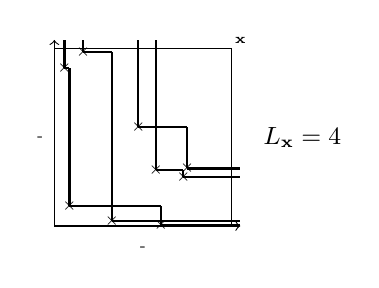
\begin{tikzpicture}[x=0.45mm,y=0.45mm,scale=0.5]
    \draw[->](0,0)--(105,0);
    \draw[->](0,0)--(0,105);
    \draw(100,0)--(100,100)--(0,100);
    \draw(105,105)node{\tiny\(\mathbf x\)};
    
    \draw(140,50)node{\small\(L_\mathbf x=4\)};
  
    \draw(8.5,11.3)node{\tiny\(\times\)};
    \draw(32.5,2.8)node{\tiny\(\times\)};
    \draw(60.1,0.7)node{\tiny\(\times\)};
    \draw(57.3,31.8)node{\tiny\(\times\)};
    \draw(5.7,89.1)node{\tiny\(\times\)};
    \draw(72.8,27.6)node{\tiny\(\times\)};
    \draw(47.4,55.9)node{\tiny\(\times\)};
    \draw(75,32.5)node{\tiny\(\times\)};
    \draw(16.3,98.3)node{\tiny\(\times\)};
  
    %1.
    \draw[thick](5.7,89.1)--(5.7,105);
    \draw[thick](5.7,89.1)--(8.5,89.1);
  
    %2.
    \draw[thick](8.5,11.3)--(8.5,89.1);
    \draw[thick](8.5,11.3)--(60.1,11.3);
  
    %3.
    \draw[thick](16.3,98.3)--(16.3,105);
    \draw[thick](16.3,98.3)--(32.5,98.3);
  
    %4.
    \draw[thick](32.5,2.8)--(32.5,98.3);
    \draw[thick](32.5,2.8)--(105,2.8);
  
    %5.
    \draw[thick](47.4,55.9)--(47.4,105);
    \draw[thick](47.4,55.9)--(75,55.9);
  
    %6.
    \draw[thick](57.3,31.8)--(57.3,105);
    \draw[thick](57.3,31.8)--(72.8,31.8);
  
    %7.
    \draw[thick](60.1,0.7)--(60.1,11.3);
    \draw[thick](60.1,0.7)--(105,0.7);
  
    %8.
    \draw[thick](72.8,27.6)--(72.8,31.8);
    \draw[thick](72.8,27.6)--(105,27.6);
  
    %9.
    \draw[thick](75,32.5)--(75,55.9);
    \draw[thick](75,32.5)--(105,32.5);
  
    \draw(-8,50)node{\tiny-};
    \draw(50,-12)node{\tiny-};
   \end{tikzpicture}
  \end{center}
 \uncover<2->{
  \begin{theorem}
   With zero boundaries,
   \[
    \lim_{\mathbf x\to\infty}\frac{L_\mathbf x}{|\mathbf x|}=2\sqrt\frac{x_1x_2}{|\mathbf x|^2\cdot(1-t)}.
   \]
  \end{theorem}
 }
\end{frame}
\begin{frame}{Second class particles}

 \begin{minipage}[t]{0.53\textwidth}
  \vspace{0pt}
  \begin{tikzpicture}[x=0.45mm,y=0.45mm]
   \draw[->](0,0)--(105,0);
   \draw[->](0,0)--(0,105);
   \draw(100,0)--(100,100)--(0,100);
 
   \draw(8.5,11.3)node{\(\times\)};
   \draw(32.5,2.8)node{\(\times\)};
   \draw(60.1,0.7)node{\(\times\)};
   \draw(57.3,31.8)node{\(\times\)};
   \draw(5.7,89.1)node{\(\times\)};
   \draw(72.8,27.6)node{\(\times\)};
   \draw(47.4,55.9)node{\(\times\)};
   \draw(75,32.5)node{\(\times\)};
   \draw(16.3,98.3)node{\(\times\)};
 
   %1.
   \uncover<-27,30-32>{
    \draw[thick](5.7,89.1)--(5.7,105);
    \draw[thick](5.7,89.1)--(47.4,89.1);
   }
 
   %2.
   \uncover<-27,30-32>{
    \draw[thick](8.5,11.3)--(8.5,57);
    \draw[thick](8.5,11.3)--(60.1,11.3);
   }
 
   %3.
   \uncover<-27,30-32>{
    \draw[thick](16.3,98.3)--(16.3,105);
    \draw[thick](16.3,98.3)--(105,98.3);
   }

   %4.
   \uncover<-27,30-32>{
    \draw[thick](32.5,2.8)--(32.5,81);
    \draw[thick](32.5,2.8)--(105,2.8);
   }
 
   %5.
   \uncover<-27,30-32>{
    \draw[thick](47.4,55.9)--(47.4,89.1);
    \draw[thick](47.4,55.9)--(75,55.9);
   }
 
   %6.
   \uncover<-27,30-32>{
    \draw[thick](57.3,31.8)--(57.3,105);
    \draw[thick](57.3,31.8)--(72.8,31.8);
   }
 
   %7.
   \uncover<-27,30-32>{
    \draw[thick](60.1,0.7)--(60.1,11.3);
    \draw[thick](60.1,0.7)--(71,0.7);
   }
 
   %8.
   \uncover<-27,30-32>{
    \draw[thick](72.8,27.6)--(72.8,31.8);
    \draw[thick](72.8,27.6)--(105,27.6);
   }
 
   %9.
   \uncover<-27,30-32>{
    \draw[thick](75,32.5)--(75,55.9);
    \draw[thick](75,32.5)--(105,32.5);
   }


   %B0
    \uncover<4-5>{
     \draw[thick,red](17,-5)--(17,0);
    }
    \uncover<6-7>{
     \draw[thick,red](17,-5)--(17,11.3);
    }
    \uncover<8-9>{
     \draw[thick,red](17,-5)--(17,16.3);
    }
    \uncover<10-30,32>{
     \draw[thick,red](17,-5)--(17,39);
    }
    \uncover<12-30,32>{
     \foreach\x in{18,19,...,21}
      \draw[red](\x-1,41)--(\x+1,37);
    }
    \uncover<12-15>{
     \draw[thick,red](22,39)--(22,44);
    }
    \uncover<16-17>{
     \draw[thick,red](22,39)--(22,89.1);
    }
    \uncover<18-30,32>{
     \draw[thick,red](22,39)--(22,94.1);
    }
    \uncover<22-23>{
     \draw[thick,red](22,39)--(22,98.3);
    }
    \uncover<24-30,32>{
     \draw[thick,red](22,39)--(22,105);
    }
    \uncover<29-30,32>{
     \draw(17,-8)node{\tiny\alert1};
    }
    \uncover<29-30,32>{
     \draw(22,108)node{\tiny\alert0};
    }

   %B1
   \uncover<-27,30-32>{
    \draw[thick](22,-5)--(22,39);
   }

   %B2
   \uncover<-27,30-32>{
    \draw[thick](71,-5)--(71,0.7);
   }

   %L1
   \uncover<-27,30-32>{
    \draw[thick](-5,39)--(22,39);
   }

   %L2
   \uncover<-27,30-32>{
    \draw[thick](-5,57)--(8.5,57);
   }
    \uncover<5-8>{
     \foreach\x in{-4,-3,...,-1}
      \draw[red](\x-1,59)--(\x+1,55);
    }
    \uncover<9-30,32>{
     \foreach\x in{-4,-3,...,7}
      \draw[red](\x-1,59)--(\x+1,55);
    }
    \only<9-12>{
     \draw[thick,red](8.5,57)--(8.5,62);
    }
    \only<13-30,32>{
     \draw[thick,red](8.5,57)--(8.5,81);
    }
    \uncover<15-30,32>{
     \foreach\x in{9,10,...,32}
      \draw[red](\x-1,83)--(\x+1,79);
    }
    \only<15-18>{
     \draw[thick,red](32.5,81)--(32.5,86);
    }
    \only<19-30,32>{
     \draw[thick,red](32.5,81)--(32.5,89.1);
    }
    \uncover<21-30,32>{
     \foreach\x in{33,34,...,47}
      \draw[red](\x-1,91.1)--(\x+1,87.1);
    }
    \only<21-24>{
     \draw[thick,red](47.4,89.1)--(47.4,94.1);
    }
    \only<25-30,32>{
     \draw[thick,red](47.4,89.1)--(47.4,98.3);
    }
    \uncover<27-30,32>{
     \foreach\x in{48,49,...,104}
      \draw[red](\x-1,100.3)--(\x+1,96.3);
    }

    \uncover<29-30,32>{
     \draw(-6,57)node{\tiny\alert0};
    }
    \uncover<29-30,32>{
     \draw(106,98.3)node{\tiny\alert1};
    }

   %L3
   \uncover<-27,30-32>{
    \draw[thick](-5,81)--(32.5,81);
   }

   \uncover<7>{
    \draw(17,11.3)node{\includegraphics[width=7mm]{head_tr.png}};
   }

   \uncover<11>{
    \draw(17,39)node{\includegraphics[width=7mm]{tail_tr.png}};
   }

   \uncover<14>{
    \draw(8.5,81)node{\includegraphics[width=7mm]{tail_tr.png}};
   }

   \uncover<17>{
    \draw(22,89.1)node{\includegraphics[width=7mm]{head_tr.png}};
   }

   \uncover<20>{
    \draw(32.5,89.1)node{\includegraphics[width=7mm]{tail_tr.png}};
   }

   \uncover<23>{
    \draw(22,98.3)node{\includegraphics[width=7mm]{head_tr.png}};
   }

   \uncover<26>{
    \draw(47.4,98.3)node{\includegraphics[width=7mm]{tail_tr.png}};
   }

   \uncover<33->{
    \draw[blue,thick](-5,39)--(17,39)--(17,-5);
    \draw[blue,thick](-5,81)--(8.5,81)--(8.5,11.3)--(60.1,11.3)--(60.1,11.3)--(60.1,0.7)--(71,0.7)--(71,-5);
    \draw[blue,thick](5.7,105)--(5.7,89.1)--(32.5,89.1)--(32.5,2.8)--(105,2.8);
    \draw[blue,thick](16.3,105)--(16.3,98.3)--(47.4,98.3)--(47.4,55.9)--(75,55.9)--(75,32.5)--(105,32.5);
    \draw[blue,thick](22,105)--(22,-5);
    \draw[blue,thick](57.3,105)--(57.3,31.8)--(72.8,31.8)--(72.8,27.6)--(105,27.6);
   }
  \end{tikzpicture}
 \end{minipage}
 \begin{minipage}[t]{0.45\textwidth}
  \vspace{0pt}
  \alt<2->{
   Definition: \(\al\le\structure{\om}\), if
  }
  {
   \phantom{Definition: }\(\al\phantom{\le\om}\)
  }
  \uncover<2->{
   \begin{itemize}
    \item more verticals in \(\structure{\om}\),
    \item more horizontals in \(\al\).
    \item<3-> \expl{(less horizontals in \(\structure{\om}\).)}
   \end{itemize}
  }

  \hop
  \uncover<28->{
  \noindent
   \(\frac{\structure\om}{\al}\) \alert{second class particles:

   upright paths}
  }

  \uncover<29->{
   \alert{that stay ordered}
  }
 \end{minipage}
\end{frame}

\section{Proof}

\begin{frame}{The main actors}

 \begin{minipage}[t]{0.53\textwidth}
  \vspace{0pt}
  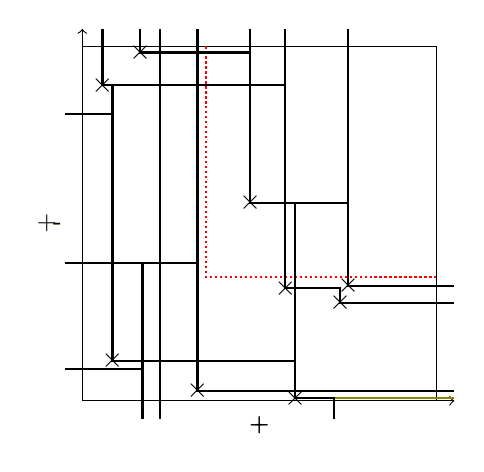
\begin{tikzpicture}[x=0.45mm,y=0.45mm]
   \draw[->](0,0)--(105,0);
   \draw[->](0,0)--(0,105);
   \draw(100,0)--(100,100)--(0,100);
 
   \draw(8.5,11.3)node{\(\times\)};
   \draw(32.5,2.8)node{\(\times\)};
   \draw(60.1,0.7)node{\(\times\)};
   \draw(57.3,31.8)node{\(\times\)};
   \draw(5.7,89.1)node{\(\times\)};
   \draw(72.8,27.6)node{\(\times\)};
   \draw(47.4,55.9)node{\(\times\)};
   \draw(75,32.5)node{\(\times\)};
   \draw(16.3,98.3)node{\(\times\)};
 
   \uncover<1>{
    \draw[olive,thick](5.7,105)--(5.7,89.1)--(8.5,89.1)--(8.5,11.3)--(60.1,11.3)--(60.1,11.3)--(60.1,0.7)--(71,0.7)--(105,0.7);
    \draw[olive,thick](16.3,105)--(16.3,98.3)--(32.5,98.3)--(32.5,2.8)--(105,2.8);
    \draw[olive,thick](47.4,105)--(47.4,55.9)--(75,55.9)--(75,32.5)--(105,32.5);
    \draw[olive,thick](57.3,105)--(57.3,31.8)--(72.8,31.8)--(72.8,27.6)--(105,27.6);
    \draw[olive](-7,50)node{\small-};
    \draw[olive](50,-7)node{\small-};
    \draw[red,thick,densely dotted](35,100)--(35,35)--(100,35);
   }

   \uncover<2>{
    \draw[thick](5.7,105)--(5.7,89.1)--(8.5,89.1)--(8.5,11.3)--(17,11.3)--(17,-5);
    \draw[thick](16.3,105)--(16.3,98.3)--(22,98.3)--(22,-5);
    \draw[thick](32.5,105)--(32.5,2.8)--(105,2.8);
    \draw[thick](47.4,105)--(47.4,55.9)--(60.1,55.9)--(60.1,11.3)--(60.1,0.7)--(71,0.7)--(71,-5);
    \draw[thick](75,105)--(75,32.5)--(105,32.5);
    \draw[thick](57.3,105)--(57.3,31.8)--(72.8,31.8)--(72.8,27.6)--(105,27.6);
    \draw(-7,50)node{\small-};
    \draw(50,-7)node{\small\(\la+\ve\)};
   }

   \uncover<3>{
    \draw[thick](-5,39)--(17,39)--(17,-5);
    \draw[thick](-5,81)--(8.5,81)--(8.5,11.3)--(60.1,11.3)--(60.1,11.3)--(60.1,0.7)--(71,0.7)--(71,-5);
    \draw[thick](5.7,105)--(5.7,89.1)--(32.5,89.1)--(32.5,2.8)--(105,2.8);
    \draw[thick](16.3,105)--(16.3,98.3)--(47.4,98.3)--(47.4,55.9)--(75,55.9)--(75,32.5)--(105,32.5);
    \draw[thick](22,105)--(22,-5);
    \draw[thick](57.3,105)--(57.3,31.8)--(72.8,31.8)--(72.8,27.6)--(105,27.6);
    \draw(-10,50)node{\small\(\la+\ve\)};
    \draw(50,-7)node{\small\(\la+\ve\)};
   }

   \uncover<4->{
    \draw[thick](-5,9)--(17,9)--(17,-5);
    \draw[thick](-5,39)--(32.5,39)--(32.5,2.8)--(105,2.8);
    \draw[thick](-5,81)--(8.5,81)--(8.5,11.3)--(60.1,11.3)--(60.1,11.3)--(60.1,0.7)--(71,0.7)--(71,-5);
    \draw[thick](5.7,105)--(5.7,89.1)--(57.3,89.1)--(57.3,31.8)--(72.8,31.8)--(72.8,27.6)--(105,27.6);;
    \draw[thick](16.3,105)--(16.3,98.3)--(47.4,98.3)--(47.4,55.9)--(75,55.9)--(75,32.5)--(105,32.5);
    \draw(-7,50)node{\small\(\la\)};
    \draw(50,-7)node{\small\(\la\)};
   }
  \end{tikzpicture}
 \end{minipage}
 \begin{minipage}[t]{0.45\textwidth}
  \vspace{0pt}
  WTS: no.\ of lines crossing
  \begin{tikzpicture}[x=0.45mm,y=0.45mm]
   \draw[red,thick,densely dotted](10,0)--(0,0)--(0,10);
  \end{tikzpicture}
  \(\to\) stati(\(\la(\mathbf v)\)) Poisson


  \hop
  \(\olgr{\te^{-,-}}
  \uncover<2->{
   \le\om^{\la+\ve,-}
  }\)

  \hop
  \(\uncover<2->{
   \om^{\la+\ve,-}
  }
  \uncover<3->{
   \ge\eta^{\la+\ve,\la+\ve}
  }
  \uncover<4->{
   \ge\al^{\la,\la}
  }\)
 \end{minipage}
  
 \vfill
 \uncover<5->{
  \hrule
 }

\vskip5pt\noindent
 \uncover<5->{
  \small{\(\olgr{\te^{-,-}}\le\om^{\la+\ve,-}\ge\eta^{\la+\ve,\la+\ve}\ge\al^{\la,\la}\)}
 }

\end{frame}

\begin{frame}{1. \(\frac{\om^{\la+\ve,-}}{\al^{\la,\la}}\) 2nd class particles and the small box}

 \begin{minipage}[t]{0.53\textwidth}
  \vspace{0pt}
  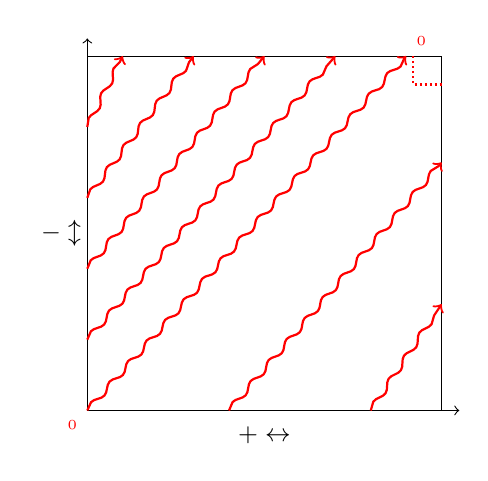
\begin{tikzpicture}[x=0.45mm,y=0.45mm]
   \draw[->](0,0)--(105,0);
   \draw[->](0,0)--(0,105);
   \draw(100,0)--(100,100)--(0,100);
 
   \draw[red,thick,decorate,decoration={snake,amplitude=1},->](0,80)--(10,100);
   \draw[red,thick,decorate,decoration={snake,amplitude=1},->](0,60)--(30,100);
   \draw[red,thick,decorate,decoration={snake,amplitude=1},->](0,40)--(50,100);
   \draw[red,thick,decorate,decoration={snake,amplitude=1},->](0,20)--(70,100);
   \draw[red,thick,decorate,decoration={snake,amplitude=1},->](0,0)node[below left]{\tiny0}--(90,100)node[above right]{\tiny0};
   \draw[red,thick,decorate,decoration={snake,amplitude=1},->](40,0)--(100,70);
   \draw[red,thick,decorate,decoration={snake,amplitude=1},->](80,0)--(100,30);

   \draw[red,thick,densely dotted](92,100)--(92,92)--(100,92);

   \draw(-7,50)node{\small\(\begin{matrix}-\\\updownarrow\\\la\end{matrix}\)};
   \draw(50,-7)node{\small\(\la+\ve\leftrightarrow\la\)};
  \end{tikzpicture}
 \end{minipage}
 \begin{minipage}[t]{0.45\textwidth}
  \vspace{0pt}
  Second class particle 0 goes above the small box.

  \hop
  \uncover<2->{
   That's because of the shape thm for each \(\om^{\la+\ve,-}\) and \(\al^{\la,\la}\),

   \hop
   and the \(\ve\) leeway.
  }
 \end{minipage}
  \vfill
  \hrule

 \vskip5pt\noindent
 \small{\(\olgr{\te^{-,-}}\le\un{\om^{\la+\ve,-}}\ge\eta^{\la+\ve,\la+\ve}\ge\un{\al^{\la,\la}}\)}

\end{frame}

\begin{frame}{2. \(\frac{\om^{\la+\ve,-}}{\eta^{\la+\ve,\la+\ve}}\) on \(\frac{\om^{\la+\ve,-}}{\al^{\la,\la}}\)}

 \begin{minipage}[t]{0.53\textwidth}
  \vspace{0pt}
  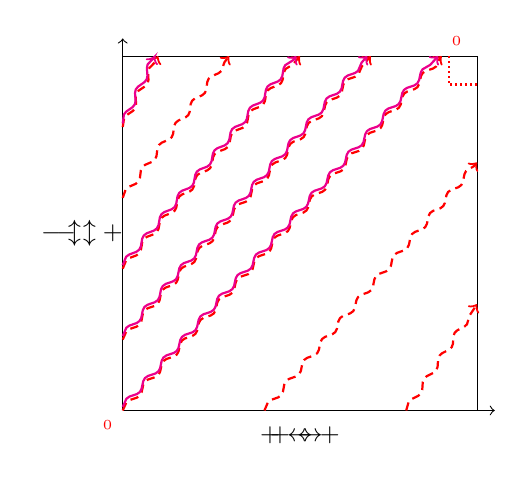
\begin{tikzpicture}[x=0.45mm,y=0.45mm]
   \draw[->](0,0)--(105,0);
   \draw[->](0,0)--(0,105);
   \draw(100,0)--(100,100)--(0,100);
 
   \draw[densely dashed,red,thick,decorate,decoration={snake,amplitude=1},->](0,80)--(10,100);
   \draw[densely dashed,red,thick,decorate,decoration={snake,amplitude=1},->](0,60)--(30,100);
   \draw[densely dashed,red,thick,decorate,decoration={snake,amplitude=1},->](0,40)--(50,100);
   \draw[densely dashed,red,thick,decorate,decoration={snake,amplitude=1},->](0,20)--(70,100);
   \draw[densely dashed,red,thick,decorate,decoration={snake,amplitude=1},->](0,0)node[below left]{\tiny0}--(90,100)node[above right]{\tiny0};
   \draw[densely dashed,red,thick,decorate,decoration={snake,amplitude=1},->](40,0)--(100,70);
   \draw[densely dashed,red,thick,decorate,decoration={snake,amplitude=1},->](80,0)--(100,30);

   \only<2->{
    \draw[magenta,thick,decorate,decoration={snake,amplitude=1},->](0,81)--(9,100);
    \draw[magenta,thick,decorate,decoration={snake,amplitude=1},->](0,41)--(49,100);
    \draw[magenta,thick,decorate,decoration={snake,amplitude=1},->](0,21)--(69,100);
    \draw[magenta,thick,decorate,decoration={snake,amplitude=1},->](0,1)--(89,100);
   }

   \draw[red,thick,densely dotted](92,100)--(92,92)--(100,92);

   \alt<2->{
    \draw(-10,50)node{\small\(\begin{matrix}-\\\updownarrow\\\la+\ve\end{matrix}\)};
    \draw(50,-7)node{\small\(\la+\ve\leftrightarrow\la+\ve\)};
   }
   {
    \draw(-17,50)node{\small\(\begin{matrix}-\\\updownarrow\\\la\end{matrix}\)};
    \draw(50,-7)node{\small\(\la+\ve\leftrightarrow\la\phantom{\ve}\)};
   }
  \end{tikzpicture}
 \end{minipage}
 \begin{minipage}[t]{0.45\textwidth}
  \vspace{0pt}
  \uncover<2->{
   \(\Bigl\{\frac{\om^{\la+\ve,-}}{\eta^{\la+\ve,\la+\ve}}\Bigr\}\subseteq\Bigl\{\frac{\om^{\la+\ve,-}}{\al^{\la,\la}}\Bigr\}\)

   \hop
   and only start from the left boundary.
  }

  \hop
  \uncover<3->{
   \(\leadsto\) there is a rightmost \(\frac{\om^{\la+\ve,-}}{\eta^{\la+\ve,\la+\ve}}\) second class particle, jumping on \(\Bigl\{\frac{\om^{\la+\ve,-}}{\al^{\la,\la}}\Bigr\}\).
  }
 \end{minipage}
  \vfill
  \hrule

 \vskip5pt\noindent
 \alt<2->{
  \small{\(\olgr{\te^{-,-}}\le\un{\om^{\la+\ve,-}\ge\eta^{\la+\ve,\la+\ve}}\ge\al^{\la,\la}\)}
 }
 {
  \small{\(\olgr{\te^{-,-}}\le\un{\om^{\la+\ve,-}}\ge\eta^{\la+\ve,\la+\ve}\ge\un{\al^{\la,\la}}\)}
 }

\end{frame}

\begin{frame}{3. \(\frac{\om^{\la+\ve,-}}{\eta^{\la+\ve,\la+\ve}}\) on \(\frac{\om^{\la+\ve,-}}{\al^{\la,\la}}\): we have drift!}

 \begin{minipage}[t]{0.53\textwidth}
  \vspace{0pt}
  \begin{tikzpicture}[x=0.45mm,y=0.45mm]
   \draw[->](0,0)--(105,0);
   \draw[->](0,0)--(0,105);
   \draw(100,0)--(100,100)--(0,100);
 
   \uncover<-2>{
    \draw[densely dashed,red,thick,decorate,decoration={snake,amplitude=1},->](0,80)--(10,100);
    \draw[densely dashed,red,thick,decorate,decoration={snake,amplitude=1},->](0,60)--(30,100);
    \draw[densely dashed,red,thick,decorate,decoration={snake,amplitude=1},->](0,40)--(50,100);
    \draw[densely dashed,red,thick,decorate,decoration={snake,amplitude=1},->](0,20)--(70,100);
    \draw[densely dashed,red,thick,decorate,decoration={snake,amplitude=1},->](0,0)node[below left]{\tiny0}--(90,100)node[above right]{\tiny0};
    \draw[densely dashed,red,thick,decorate,decoration={snake,amplitude=1},->](40,0)--(100,70);
    \draw[densely dashed,red,thick,decorate,decoration={snake,amplitude=1},->](80,0)--(100,30);
 
    \draw[magenta,thick,decorate,decoration={snake,amplitude=1},->](0,81)--(9,100);
    \draw[magenta,thick,decorate,decoration={snake,amplitude=1},->](0,41)--(49,100);
    \draw[magenta,thick,decorate,decoration={snake,amplitude=1},->](0,21)--(69,100);
    \draw[magenta,thick,decorate,decoration={snake,amplitude=1},->](0,1)--(89,100);
 
    \draw[red,thick,densely dotted](92,100)--(92,92)--(100,92);
   }
   \only<3->{
    \foreach\x in{31,32,...,69}
     \draw[red](48,\x+1)--(52,\x-1);
    \draw[red,thick](30,50)--(70,50);
    \draw[red](27,50)node{\small0};
    \draw[red](73,50)node{\small1};
    \draw[red](50,73)node{\small0};
    \draw[red](50,27)node{\small1};
   }
   \only<4-5>{
    \foreach\x in{31,32,...,69}
     \draw[magenta](43,\x+1)--(47,\x-1);
   }
   \only<7->{
     \draw[thick,magenta](30,51)--(47,51);
   }
   \only<8>{
    \draw(50,50)node{\includegraphics[width=7mm]{head_tr.png}};
   }
   \only<9>{
     \draw[thick,magenta](47,51)--(70,51);
   }
   \only<10>{
    \draw(50,50)node{\includegraphics[width=7mm]{tail_tr.png}};
   }
   \only<11->{
    \foreach\x in{51,52,...,69}
     \draw[magenta](43,\x+1)--(47,\x-1);
   }

   \draw(-10,50)node{\small\(\begin{matrix}-\\\updownarrow\\\la+\ve\end{matrix}\)};
   \draw(50,-7)node{\small\(\la+\ve\leftrightarrow\la+\ve\)};
  \end{tikzpicture}
 \end{minipage}
 \begin{minipage}[t]{0.45\textwidth}
  \vspace{0pt}
  \(\Bigl\{\frac{\om^{\la+\ve,-}}{\eta^{\la+\ve,\la+\ve}}\Bigr\}\subseteq\Bigl\{\frac{\om^{\la+\ve,-}}{\al^{\la,\la}}\Bigr\}\)

  \hop
  \begin{tikzpicture}
   \draw[red,->](0,0)--(4,0)node[below]{\tiny\(\frac{\om^{\la+\ve,-}}{\al^{\la,\la}}\)};
   \foreach\x in{0,0.4,...,3.6}
    \draw[red](\x,-0.1)--(\x,0.1);

   \uncover<4->{
    \draw[red](2.4,-0.3)node{\small1};
    \draw[red](2,-0.3)node{\small0};
   }

   \draw[magenta](0.7,0.1)--(0.8,0.3)--(0.9,0.1);
   \draw[magenta](0.8,0.3)--(0.8,0.5);
   \draw[magenta](0.7,0.4)--(0.8,0.47)--(0.9,0.4);
   \draw[magenta](0.8,0.6)circle(0.1);
   \draw[magenta](0.77,0.63)circle(0.01);
   \draw[magenta](0.83,0.63)circle(0.01);
   \draw[magenta](0.77,0.56)arc(233:307:0.05);

   \draw[magenta](1.1,0.1)--(1.2,0.3)--(1.3,0.1);
   \draw[magenta](1.2,0.3)--(1.2,0.5);
   \draw[magenta](1.1,0.4)--(1.2,0.47)--(1.3,0.4);
   \draw[magenta](1.2,0.6)circle(0.1);
   \draw[magenta](1.17,0.63)circle(0.01);
   \draw[magenta](1.23,0.63)circle(0.01);
   \draw[magenta](1.17,0.56)arc(233:307:0.05);

   \only<-4,9>{
    \draw[magenta](2.3,0.1)--(2.4,0.3)--(2.5,0.1);
    \draw[magenta](2.4,0.3)--(2.4,0.5);
    \draw[magenta](2.3,0.4)--(2.4,0.47)--(2.5,0.4);
    \draw[magenta](2.4,0.6)circle(0.1);
    \draw[magenta](2.37,0.63)circle(0.01);
    \draw[magenta](2.43,0.63)circle(0.01);
    \draw[magenta](2.37,0.56)arc(233:307:0.05);
   }
   \only<5,7-8,10->{
    \draw[magenta](1.9,0.1)--(2,0.3)--(2.1,0.1);
    \draw[magenta](2,0.3)--(2,0.5);
    \draw[magenta](1.9,0.4)--(2,0.47)--(2.1,0.4);
    \draw[magenta](2,0.6)circle(0.1);
    \draw[magenta](1.97,0.63)circle(0.01);
    \draw[magenta](2.03,0.63)circle(0.01);
    \draw[magenta](1.97,0.56)arc(233:307:0.05);
   }

   \draw[magenta](3.1,0.1)--(3.2,0.3)--(3.3,0.1);
   \draw[magenta](3.2,0.3)--(3.2,0.5);
   \draw[magenta](3.1,0.4)--(3.2,0.47)--(3.3,0.4);
   \draw[magenta](3.2,0.6)circle(0.1);
   \draw[magenta](3.17,0.63)circle(0.01);
   \draw[magenta](3.23,0.63)circle(0.01);
   \draw[magenta](3.17,0.56)arc(233:307:0.05);
  \end{tikzpicture}

  \hip
  \(\curvearrowleft\): prob.\ 1

  \(\curvearrowright\): prob.\ \(t\)

  \hip
  \uncover<2->{
   \(\leadsto\) rightmost \(\frac{\om^{\la+\ve,-}}{\eta^{\la+\ve,\la+\ve}}\) second class still left of the small box whp.
  }
 \end{minipage}
  \vfill
  \hrule

 \vskip5pt\noindent
 \small{\(\olgr{\te^{-,-}}\le\un{\om^{\la+\ve,-}\ge\eta^{\la+\ve,\la+\ve}}\ge\al^{\la,\la}\)}

\end{frame}

\begin{frame}{4. Conclusion}

 \begin{minipage}[t]{0.53\textwidth}
  \vspace{0pt}
  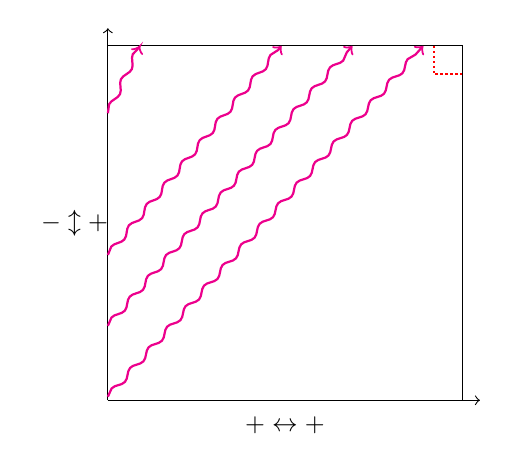
\begin{tikzpicture}[x=0.45mm,y=0.45mm]
   \draw[->](0,0)--(105,0);
   \draw[->](0,0)--(0,105);
   \draw(100,0)--(100,100)--(0,100);
 
   \draw[magenta,thick,decorate,decoration={snake,amplitude=1},->](0,81)--(9,100);
   \draw[magenta,thick,decorate,decoration={snake,amplitude=1},->](0,41)--(49,100);
   \draw[magenta,thick,decorate,decoration={snake,amplitude=1},->](0,21)--(69,100);
   \draw[magenta,thick,decorate,decoration={snake,amplitude=1},->](0,1)--(89,100);

   \draw[red,thick,densely dotted](92,100)--(92,92)--(100,92);

   \draw(-10,50)node{\small\(\begin{matrix}-\\\updownarrow\\\la+\ve\end{matrix}\)};
   \draw(50,-7)node{\small\(\la+\ve\leftrightarrow\la+\ve\)};
  \end{tikzpicture}

  \uncover<5->{
   \begin{center}
    \structure{\emph{Thank you.}}
   \end{center}
  }
 \end{minipage}
 \begin{minipage}[t]{0.45\textwidth}
  \vspace{0pt}
  Rightmost \(\frac{\om^{\la+\ve,-}}{\eta^{\la+\ve,\la+\ve}}\) second class still left of the small box whp.

  \hop
  \uncover<2->{
   \(\leadsto\ \om^{\la+\ve,-}=\eta^{\la+\ve,\la+\ve}\) in the small box whp.
  }

  \hop
  \uncover<3->{
   \(\leadsto\) but \(\eta^{\la+\ve,\la+\ve}\) is stationary so has Poi(\(\la+\ve\)) number of lines entering the box whp.
  }

  \hop
  \uncover<4->{
   \(\leadsto\) whp.\ \(\olgr{\te^{-,-}}\le\text{Poi}(\la+\ve)\) \(\forall\ve>0\).
  }
 \end{minipage}
  \vfill
  \hrule

 \vskip5pt\noindent
 \small{\(\olgr{\te^{-,-}}\le\un{\om^{\la+\ve,-}\ge\eta^{\la+\ve,\la+\ve}}\ge\al^{\la,\la}\)}

\end{frame}
%szerkbodyend

\end{document}
